%================================
%   この節の概要/内容について
%================================
本節では、まずはじめに、FDPS\describeForEach{}{および FDPS Fortranインターフェース}{および FDPS C言語インターフェース}の動作環境、必要なソフトウェア、インストール方法などを説明し、その後、サンプルコードの使用方法を説明する。サンプルコードの中身に関しては、次節(第\ref{sec:how_to_use}節)で詳しく述べる。

%%%%%%%%%%%%%%%%%%%%%%%%%%%%%%%%%%%%%%%%%%%%%%%%%%%%%
\subsection{動作環境}
FDPSはLinux, Mac OS X, WindowsなどのOS上で動作する。

%%%%%%%%%%%%%%%%%%%%%%%%%%%%%%%%%%%%%%%%%%%%%%%%%%%%%
\subsection{必要なソフトウェア}
本節では、FDPSを使用する際に必要となるソフトウェアを記述する。まず標準
機能を用いるのに必要なソフトウェア、次に拡張機能を用いるのに必要なソフ
トウェアを記述する。
%%%%%%%%%%%%%%%%%%%%%%%%%%%%%%%
\subsubsection{標準機能}
本節では、FDPSの標準機能のみを使用する際に必要なソフトウェアを記述する。
最初に逐次処理機能のみを用いる場合(並列処理機能を用いない場合)に必要
なソフトウェアを記述する。次に並列処理機能を用いる場合に必要なソフトウェ
アを記述する。
%%%%%%%%%%%%%%%%
\subsubsubsection{逐次処理}
逐次処理の場合に必要なソフトウェアは以下の通りである。
\begin{itemize}
\item make
\item C++コンパイラ(gccバージョン4.8.3以降なら確実, Kコンパイラバージョ
  ン1.2.0で動作確認済)
\describeForFtn{% Fortran版記述[開始]
\item Fortranコンパイラ (Fortran 2003 標準をサポートし、上記 C++コンパイラと相互運用可能なもの。gcc 4.8.3 以降のgfortranなら確実)
\item Python 2.7.5以上、または、Python 3.4以上 (これ以外での正常動作は保証しない。特に、Python 2.7以前では動作しない)
}%Fortran版記述[終了]
\describeForC{% C言語版記述[開始]
\item Cコンパイラ (上記 C++コンパイラと相互運用可能なもの。gcc 4.8.3 以降のgfortranなら確実)
\item Python 2.7.5以上、または、Python 3.4以上 (これ以外での正常動作は保証しない。特に、Python 2.7以前では動作しない)
}%C言語版記述[終了]

\end{itemize}
%%%%%%%%%%%%%%%%
\subsubsubsection{並列処理}
本節では、FDPSの並列処理機能を用いる際に必要なソフトウェアを記述する。
まず、OpenMPを使用する際に必要なソフトウェア、次にMPIを使用する際に必要
なソフトウェア、最後にOpenMPとMPIを同時に使用する際に必要なソフトウェア
を記述する。
%%%%%%%%
\subsubsubsubsection{OpenMP}
OpenMPを使用する際に必要なソフトウェアは以下の通り。
\begin{itemize}
\item make
\item OpenMP対応のC++コンパイラ(gcc version 4.8.3以降なら確実, Kコンパ
  イラバージョン1.2.0で動作確認済)
\describeForFtn{% Fortran版記述[開始]
\item OpenMP対応のFortranコンパイラ (Fortran 2003 標準をサポートし、上記 C++コンパイラと相互運用可能なもの。gcc 4.8.3以降なら確実)
\item Python 2.7.5以上、または、Python 3.4以上 (これ以外での正常動作は保証しない。特に、Python 2.7以前では動作しない)
}%Fortran版記述[終了]
\describeForC{% C言語版記述[開始]
\item OpenMP対応のCコンパイラ (上記 C++コンパイラと相互運用可能なもの。gcc 4.8.3以降なら確実)
\item Python 2.7.5以上、または、Python 3.4以上 (これ以外での正常動作は保証しない。特に、Python 2.7以前では動作しない)
}%C言語版記述[終了]

\end{itemize}
%%%%%%%%
\subsubsubsubsection{MPI}
MPIを使用する際に必要なソフトウェアは以下の通り。
\begin{itemize}
\item make
\item MPI version 1.3対応のC++コンパイラ(Open MPI 1.6.4で動作確認済, K
  コンパイラバージョン1.2.0で動作確認済)
\describeForFtn{%Fortran版記述[開始]
\item MPI version 1.3対応のFortranコンパイラ (Fortran 2003 標準をサポートし、上記 C++コンパイラと相互運用可能なもの。Open MPI 1.6.4で動作確認済み)
\item Python 2.7.5以上、または、Python 3.4以上 (これ以外での正常動作は保証しない。特に、Python 2.7以前では動作しない)
}%Fortran版記述[終了]
\describeForC{%C言語版記述[開始]
\item MPI version 1.3対応のCコンパイラ (上記 C++コンパイラと相互運用可能なもの。Open MPI 1.6.4で動作確認済み)
\item Python 2.7.5以上、または、Python 3.4以上 (これ以外での正常動作は保証しない。特に、Python 2.7以前では動作しない)
}%C言語版記述[終了]

\end{itemize}
%%%%%%%%
\subsubsubsubsection{MPI+OpenMP}
MPIとOpenMPを同時に使用する際に必要なソフトウェアは以下の通り。
\begin{itemize}
\item make
\item MPI version 1.3とOpenMPに対応のC++コンパイラ(Open MPI 1.6.4で動
  作確認済, Kコンパイラバージョン1.2.0で動作確認済)
\describeForFtn{%Fortran版記述[開始]
\item MPI version 1.3とOpenMPに対応のFortranコンパイラ(Fortran 2003標準をサポートし、上記 C++コンパイラと相互運用可能なもの。Open MPI 1.6.4で動作確認ずみ)
\item Python 2.7.5以上、または、Python 3.4以上 (これ以外での正常動作は保証しない。特に、Python 2.7以前では動作しない)
}%Fortran版記述[終了]
\describeForC{%C言語版記述[開始]
\item MPI version 1.3とOpenMPに対応のCコンパイラ(上記 C++コンパイラと相互運用可能なもの。Open MPI 1.6.4で動作確認ずみ)
\item Python 2.7.5以上、または、Python 3.4以上 (これ以外での正常動作は保証しない。特に、Python 2.7以前では動作しない)
}%C言語版記述[終了]

\end{itemize}
%%%%%%%%%%%%%%%%%%%%%%%%%%%%%%%
\subsubsection{拡張機能}
本節では、FDPSの拡張機能を使用する際に必要なソフトウェアについて述べる。
FDPSの拡張機能にはParticle Meshがある。以下ではParticle Meshを使用する
際に必要なソフトウェアを述べる。
%%%%%%%%%%%%%%%%
\subsubsubsection{Particle Mesh}
Particle Meshを使用する際に必要なソフトウェアは以下の通りである。
\begin{itemize}
\item make
\item MPI version 1.3とOpenMPに対応のC++コンパイラ(Open MPI 1.6.4で動
  作確認済)
\item FFTW 3.3以降
\end{itemize}

%%%%%%%%%%%%%%%%%%%%%%%%%%%%%%%%%%%%%%%%%%%%%%%%%%%%%
\subsection{インストール}
本節では、FDPS\describeForEach{}{および FDPS Fortranインターフェース}{および C言語インターフェース}のインストールについて述べる。取得方法、ビルド方法について述べる。
%%%%%%%%%%%%%%%%%%%%%%%%%%%%%%%
\subsubsection{取得方法}
ここではFDPSの取得方法を述べる。最初に最新バージョンの取得方法、次に過去のバージョンの取得方法を述べる。
%%%%%%%%%%%%%%%%
\subsubsubsection{最新バージョン}
以下の方法のいずれかでFDPSの最新バージョンを取得できる。
\begin{itemize}
\item ブラウザから
  \begin{enumerate}
  \item ウェブサイト \url{https://github.com/FDPS/FDPS}で"Download ZIP"をクリックし、ファイル\path{FDPS-master.zip}をダウンロード
  \item FDPSを展開したいディレクトリに移動し、圧縮ファイルを展開
  \end{enumerate}

\item コマンドラインから
  \begin{itemize}    
  \item Subversionを用いる場合:以下のコマンドを実行するとディレクトリ
    trunkの下をSubversionレポジトリとして使用できる
    \begin{screen}
\begin{verbatim}
$ svn co --depth empty https://github.com/FDPS/FDPS
$ cd FDPS
$ svn up trunk
\end{verbatim}
    \end{screen}

  \item Gitを用いる場合:以下のコマンドを実行するとカレントディレクト
    リにディレクトリFDPSができ、その下をGitのレポジトリとして使用できる
    \begin{screen}
\begin{verbatim}
$ git clone git://github.com/FDPS/FDPS.git
\end{verbatim}
    \end{screen}    

  \end{itemize}

\end{itemize}
%%%%%%%%%%%%%%%%
\subsubsubsection{過去のバージョン}
以下の方法でブラウザからFDPSの過去のバージョンを取得できる。
\begin{itemize}
\item ウェブサイト\url{https://github.com/FDPS/FDPS/releases}に過去のバージョ
  ンが並んでいるので、ほしいバージョンをクリックし、ダウンロード
\item FDPSを展開したいディレクトリに移動し、圧縮ファイルを展開
\end{itemize}
\if 0
\begin{itemize}
\item ブラウザから
  \begin{enumerate}
  \item ウェブサイト \url{https://github.com/FDPS/FDPS/releases}に過去のバージョンが並んでいるので、ほしいバージョンをクリックし、ダウンロード
  \item FDPSを展開したいディレクトリに移動し、圧縮ファイルを展開
  \end{enumerate}

\item コマンドラインから
  \begin{itemize}
    
  \item Gitを用いる場合:以下のコマンドを実行するとカレントディレクト
    リにディレクトリFDPSができる。
    \begin{screen}
\begin{verbatim}
$ git clone git://github.com/FDPS/FDPS.git
\end{verbatim}
    \end{screen}

    ディレクトリFDPSに移動し、以下のコマンドを実行すると、存在するFDPS
    の過去のバージョンがわかる。以下では、v0.1, v0.2, v1.0というバージョ
    ンが存在していることになる。
    \begin{screen}
\begin{verbatim}
$ git tag
v0.1
v0.2
v1.0
\end{verbatim}
    \end{screen}

    以下のコマンドを実行すると、ダウンロードしたFDPSがv0.1バージョンに
    なっている。ここではブランチを切らない場合を示す。
    \begin{screen}     
\begin{verbatim}
$ git checkout refs/tags/v0.1
\end{verbatim}
    \end{screen}

  \end{itemize}

\end{itemize}
\fi
%%%%%%%%%%%%%%%%%%%%%%%%%%%%%%%
\subsubsection{インストール方法}
\describeForCpp{%C++版記述
\texttt{configure}などをする必要はない。
}
\ifIF %Fortran,C版記述
C++言語で記述されたFDPS本体はヘッダライブラリ\footnote{ヘッダファイルだけで構成されるライブラリのこと}のため、\texttt{configure}などを行う必要はない。基本的にはアーカイブを展開したあと、自分のソースファイルをコンパイルする時に適切なインクルードパスを設定すればよい。実際の手続きは第\ref{subsec:usage_of_sample_codes}節で説明するサンプルコードとその Makefile をみて欲しい。

\progLangName の場合、コンパイル前に \progLangName ソースファイルからFDPSとのインターフェースコードを生成する必要がある。その手順は仕様書\href{file://./doc_specs_ftn_ja.pdf}{doc\_spec\_ftn\_ja.pdf}の第6章に記述されている。本サンプルコードのMakefileでは、インターフェースコードが \texttt{make} コマンド実行中に自動的に生成されるようになっている。ユーザが自分のコードの Makefile を作る時にはサンプルコードの Makefile を参考にすることを推奨する。
\endifIF


%%%%%%%%%%%%%%%%%%%%%%%%%%%%%%%%%%%%%%%%%%%%%%%%%%%%%
\subsection{サンプルコードの使用方法}
\label{subsec:usage_of_sample_codes}
本節ではサンプルコードの使用方法について説明する。サンプルコードには重力$N$体シミュレーションコードと、SPHシミュレーションコードがある。最初に重力$N$体シミュレーションコード、次にSPHシミュレーションコードの使用について記述する。サンプルコードは拡張機能を使用していない。
%%%%%%%%%%%%%%%%%%%%%%%%%%%%%%%
\subsubsection{重力$N$体シミュレーションコード}
\label{subsubsec:usage_of_sample_codes:nbody}
本サンプルコードは、\describeForEach{FDPS}{FDPS Fortranインターフェース}{FDPS C言語インターフェース}を用いて書かれた無衝突系の$N$体計算コードである。このコードでは一様球のコールドコラプス問題を計算し、粒子分布のスナップショットを出力する。
%%%%%%%%%%%%%%%%
\subsubsubsection{概要}
以下の手順で本コードを使用できる。
\begin{itemize}
\item ディレクトリ\dirNameNbodySample に移動。これ以後、ディレクトリ\texttt{\$(FDPS)}はFDPSの最も上の階層のディレクトリを指す(\texttt{\$(FDPS)}は環境変数にはなっていない)。\texttt{\$(FDPS)}はFDPSの取得によって異なり、ブラウザからならFDPS-master, Subversionからならtrunk, GitからならFDPSである。
\item カレントディレクトリにある\texttt{Makefile}を編集
\item コマンドライン上で\texttt{make}を実行
\item \texttt{nbody.out} ファイルの実行
\item 結果の解析
\end{itemize}
最後にx86版Phantom-GRAPEおよびPIKGを使う場合について述べる。

%%%%%%%%%%%%%%%%
\subsubsubsection{ディレクトリ移動}
ディレクトリ\dirNameNbodySample に移動する。

%%%%%%%%%%%%%%%%
\subsubsubsection{Makefileの編集}
\label{s3sec:how_to_edit_Makefile_in_nbody}
\ifCpp%C++用
\texttt{Makefile}の編集項目は以下の通りである。OpenMPとMPIを使用するかどうかで編集方法が変ることに注意。
\endifCpp
\ifFtn%Fortran用
サンプルコードのディレクトリには2つのMakefileがある。1つはGCC用に書かれた\texttt{Makefile}であり、もう1つはIntelコンパイラ用に書かれた\texttt{Makefile.intel}である。ここでは\texttt{Makefile}について詳しく解説し、\texttt{Makefile.intel}に関しては使用上の注意点を本節最後で述べるのみとする。

まず、\texttt{Makefile}の初期設定について説明する。サンプルコードをコンパイルするにあたって、ユーザが設定すべきMakefile変数は4つあり、Fortranコンパイラを表す\texttt{FC}、C++コンパイラを表す\texttt{CXX}、それぞれのコンパイルオプションを表す\texttt{FCFLAGS}, \texttt{CXXFLAGS}である。これらの初期設定値は次のようになっている:
\begin{screen}
\begin{Verbatim}[commandchars=\\\{\}]
FC=gfortran
CXX=g++
FCFLAGS = -std=f2003 -O3 -ffast-math -funroll-loops -finline-functions
CXXFLAGS = -O3 -ffast-math -funroll-loops \$(FDPS_INC)
\end{Verbatim}
\end{screen}
ここで、\texttt{\$(FDPS\_INC)}はFDPS本体をインクルードするために必要なインクルードPATHが格納された変数であり、\texttt{Makefile}内で設定済みである。したがって、ここで変更する必要はない。

上記4つのMakefile変数の値を適切に編集し、\texttt{make}コマンドを実行することで実行ファイルが得られる。OpenMPとMPIを使用するかどうかで編集方法が変わるため、以下でそれを説明する。
\endifFtn
\ifC%C言語用
サンプルコードのディレクトリにはGCC用に書かれた\texttt{Makefile}がある。以下、この\texttt{Makefile}について解説する。

まず、\texttt{Makefile}の初期設定について説明する。サンプルコードをコンパイルするにあたって、ユーザが設定すべきMakefile変数は4つあり、Cコンパイラを表す\texttt{CC}、C++コンパイラを表す\texttt{CXX}、それぞれのコンパイルオプションを表す\texttt{CFLAGS}, \texttt{CXXFLAGS}である。これらの初期設定値は次のようになっている:
\begin{screen}
\begin{Verbatim}[commandchars=\\\{\}]
CC=gcc
CXX=g++
CFLAGS = -O3 -ffast-math -funroll-loops -finline-functions \$(FDPS_INC)
CXXFLAGS = -O3 -ffast-math -funroll-loops \$(FDPS_INC)
\end{Verbatim}
\end{screen}
ここで、\texttt{\$(FDPS\_INC)}はFDPS本体をインクルードするために必要なインクルードPATHが格納された変数であり、\texttt{Makefile}内で設定済みである。したがって、ここで変更する必要はない。

上記4つのMakefile変数の値を適切に編集し、\texttt{make}コマンドを実行することで実行ファイルが得られる。OpenMPとMPIを使用するかどうかで編集方法が変わるため、以下でそれを説明する。
\endifC

\begin{itemize}
%%% OpenMPもMPIも使用しない場合 %%%
\item OpenMPもMPIも使用しない場合
\begin{itemize}
\describeForEach{%C++用
\item 変数\texttt{CC}にC++コンパイラを代入する
}{%Fortran用
\item 変数\texttt{FC}にFortranコンパイラを代入する
\item 変数\texttt{CXX}にC++コンパイラを代入する
}{%C言語用
\item 変数\texttt{CC}にCコンパイラを代入する
\item 変数\texttt{CXX}にC++コンパイラを代入する
}
\end{itemize}
%%% OpenMPのみ使用の場合 %%%
\item OpenMPのみ使用の場合
\begin{itemize}
\describeForEach{%C++用
\item 変数\texttt{CC}にOpenMP対応のC++コンパイラを代入する
\item \texttt{CFLAGS += -DPARTICLE\_SIMULATOR\_THREAD\_PARALLEL -fopenmp}の行のコメントアウトを外す。Intelコンパイラの場合には、\texttt{-fopenmp}を\texttt{-qopenmp}か\texttt{-openmp}に変更する(どちらを指定すべきかはコンパイラのバージョンに依る)。
}{%Fortran用
\item 変数\texttt{FC}にOpenMP対応のFortranコンパイラを代入する
\item 変数\texttt{CXX}にOpenMP対応のC++コンパイラを代入する
\item \texttt{FCFLAGS += -DPARTICLE\_SIMULATOR\_THREAD\_PARALLEL -fopenmp}の行のコメントアウトを外す
\item \texttt{CXXFLAGS += -DPARTICLE\_SIMULATOR\_THREAD\_PARALLEL -fopenmp}の行のコメントアウトを外す
}{%C言語用
\item 変数\texttt{CC}にOpenMP対応のCコンパイラを代入する
\item 変数\texttt{CXX}にOpenMP対応のC++コンパイラを代入する
\item \texttt{CFLAGS += -DPARTICLE\_SIMULATOR\_THREAD\_PARALLEL -fopenmp}の行のコメントアウトを外す
\item \texttt{CXXFLAGS += -DPARTICLE\_SIMULATOR\_THREAD\_PARALLEL -fopenmp}の行のコメントアウトを外す
}

\end{itemize}
%%% MPIのみ使用の場合 %%%
\item MPIのみ使用の場合
\begin{itemize}
\describeForEach{% C++用
\item 変数\texttt{CC}にMPI対応のC++コンパイラを代入する
\item \texttt{CFLAGS += -DPARTICLE\_SIMULATOR\_MPI\_PARALLEL}の行のコメントアウトを外す
}{% Fortran用
\item 変数\texttt{FC}にMPI対応のFortranコンパイラを代入する
\item 変数\texttt{CXX}にMPI対応のC++コンパイラを代入する
\item \texttt{FCFLAGS += -DPARTICLE\_SIMULATOR\_MPI\_PARALLEL}の行のコメントアウトを外す
\item \texttt{CXXFLAGS += -DPARTICLE\_SIMULATOR\_MPI\_PARALLEL}の行のコメントアウトを外す
}{%C言語用
\item 変数\texttt{CC}にMPI対応のCコンパイラを代入する
\item 変数\texttt{CXX}にMPI対応のC++コンパイラを代入する
\item \texttt{CFLAGS += -DPARTICLE\_SIMULATOR\_MPI\_PARALLEL}の行のコメントアウトを外す
\item \texttt{CXXFLAGS += -DPARTICLE\_SIMULATOR\_MPI\_PARALLEL}の行のコメントアウトを外す
}
\end{itemize}
%%% OpenMPとMPIの同時使用の場合 %%%
\item OpenMPとMPIの同時使用の場合
\begin{itemize}
\describeForEach{% C++用
\item 変数\texttt{CC}にMPI対応のC++コンパイラを代入する
\item \texttt{CFLAGS += -DPARTICLE\_SIMULATOR\_THREAD\_PARALLEL -fopenmp}の行のコメントアウトを外す。Intelコンパイラの場合には、\texttt{-fopenmp}を\texttt{-qopenmp}か\texttt{-openmp}に変更する(どちらを指定すべきかはコンパイラのバージョンに依る)。
\item \texttt{CFLAGS += -DPARTICLE\_SIMULATOR\_MPI\_PARALLEL}の行のコメントアウトを外す
}{% Fortran用
\item 変数\texttt{FC}にMPI対応のFortranコンパイラを代入する
\item 変数\texttt{CXX}にMPI対応のC++コンパイラを代入する
\item \texttt{FCFLAGS += -DPARTICLE\_SIMULATOR\_THREAD\_PARALLEL -fopenmp}の行のコメントアウトを外す
\item \texttt{FCFLAGS += -DPARTICLE\_SIMULATOR\_MPI\_PARALLEL}の行のコメントアウトを外す
\item \texttt{CXXFLAGS += -DPARTICLE\_SIMULATOR\_THREAD\_PARALLEL -fopenmp}の行のコメントアウトを外す
\item \texttt{CXXFLAGS += -DPARTICLE\_SIMULATOR\_MPI\_PARALLEL}の行のコメントアウトを外す
}{%C言語用
\item 変数\texttt{CC}にMPI対応のCコンパイラを代入する
\item 変数\texttt{CXX}にMPI対応のC++コンパイラを代入する
\item \texttt{CFLAGS += -DPARTICLE\_SIMULATOR\_THREAD\_PARALLEL -fopenmp}の行のコメントアウトを外す
\item \texttt{CFLAGS += -DPARTICLE\_SIMULATOR\_MPI\_PARALLEL}の行のコメントアウトを外す
\item \texttt{CXXFLAGS += -DPARTICLE\_SIMULATOR\_THREAD\_PARALLEL -fopenmp}の行のコメントアウトを外す
\item \texttt{CXXFLAGS += -DPARTICLE\_SIMULATOR\_MPI\_PARALLEL}の行のコメントアウトを外す
}
\end{itemize}
\end{itemize}

\ifFtn % Fortran用
次に、ユーザが本Makefileをユーザコードで使用する場合に便利な情報を記述する。ユーザコードで使用する場合に最も重要となるMakefile変数は、\texttt{FDPS\_LOC}, \newline \texttt{SRC\_USER\_DEFINED\_TYPE},   \texttt{SRC\_USER} の3つである。まず、変数\texttt{FDPS\_LOC}には、FDPSのトップディレクトリのPATHを格納する。本Makefileでは、FDPSのソースディレクトリのPATHやFortranとのインターフェースコードを生成するスクリプトのPATH等、FDPSに関連する各種な設定がこの変数の値に基いて自動的に設定されるようになっている。したがって、ユーザは適切に設定する必要がある。次に、変数\texttt{SRC\_USER\_DEFINED\_TYPE}, \texttt{SRC\_USER}には、それぞれ、ユーザ定義型が記述されたFortranファイル名と、ユーザ定義型以外の部分が記述されたFortranファイル名を格納する。FDPS の Fortran インターフェースコードはユーザーコードのクラス(派生型)を記述する部分から生成されるので、その部分が記述されたファイルを\texttt{SRC\_USER\_DEFINED\_TYPE}で、それ以外を\texttt{SRC\_USER}で指定する。これにより、\texttt{SRC\_USER}で指定したファイルが変更されても FDPS の再コンパイルは起きなくなるので、コンパイル・リンクの時間が短くなる。但し、\texttt{SRC\_USER\_DEFINED\_TYPE}、或いは、\texttt{SRC\_USER}に格納された(複数の)ファイルの間に依存関係がある場合、依存関係を示すルールをMakefileに追記しなければならない点に注意して頂きたい。この記述方法に関しては、例えば、GNU make のマニュアル等を読んで頂きたい。

最後に、\texttt{Makefile.intel}を使用する上での注意点について説明する。変数の初期値が異なる点を除き、\texttt{Makefile.intel}の構造は\texttt{Makefile}と同じである。したがって、変数の値をユーザが利用する計算機システムにおける値に適切に設定すれば、\texttt{Makefile}と同様に利用可能である。以下に変更する上での注意点を述べる:
\begin{itemize}[leftmargin=*]
\item \texttt{/opt/intel/bin}を、利用する計算機システムにおけるIntelコンパイラの格納ディレクトリのPATHに変更する。
\item \texttt{/opt/intel/include}を、Intelコンパイラに付属するヘッダファイル群を格納したディレクトリのPATHに変更する。
\item \texttt{Makefile.intel}の\texttt{LDFLAGS}は、\texttt{-L/opt/intel/lib/intel64 -L/usr/lib64 -lifport -lifcore -limf -lsvml -lm -lipgo -lirc -lirc\_s}となっている。\newline この中の \texttt{-lifcore} \protect\footnote{\texttt{libifcore}は、Fortran ランタイムライブラリである。}は、C++コンパイラでC++オブジェクトとFortranオブジェクトをリンクするため必要である\footnote{Intelコンパイラ(バージョン17.0.0 20160721)において確認。}。計算機システムのライブラリパスに、Intelコンパイラのライブラリ群が登録されていない場合、さらに、\texttt{-L/opt/intel/lib/intel64 -L/usr/lib64 -lifport -limf -lsvml -lm -lipgo -lirc -lirc\_s} のような指定が必要である。\newline ここで、\texttt{/opt/intel/lib/intel64}は、Intelコンパイラのライブラリ群が格納されたディレクトリのPATHで、\texttt{/usr/lib64}はライブラリ\texttt{libm}を格納したディレクトリのPATHである。これらは利用する計算機システムに合わせて修正する必要がある。コンパイルに必要なライブラリ群(\texttt{-l*})は、Intelコンパイラのバージョンによって変わる可能性があるので確認して頂きたい。
\item 本書を執筆時点(2016/12/26)で、IntelコンパイラでOpenMPを有効にするオプションは\texttt{-openmp}、或いは、\texttt{-qopenmp}である。これはIntelコンパイラのバージョンによって異なり、より新しいバージョンのコンパイラは後者を使用する(前者を使用した場合、廃止予定の警告が出る)。
\item 利用する計算機システムによっては、\texttt{-lifcore}の指定以外の設定が環境変数(\texttt{PATH}, \texttt{CPATH}, \texttt{LD\_LIBRARY\_PATH}等として)で既に行われていることもありえる。
\end{itemize}
\endifFtn
\ifC %C言語用
次に、ユーザが本Makefileをユーザコードで使用する場合に便利な情報を記述する。ユーザコードで使用する場合に最も重要となるMakefile変数は、\texttt{FDPS\_LOC}, \newline \texttt{HDR\_USER\_DEFINED\_TYPE}, \texttt{SRC\_USER} の3つである。まず、変数\texttt{FDPS\_LOC}には、FDPSのトップディレクトリのPATHを格納する。本Makefileでは、FDPSのソースディレクトリのPATHやC言語とのインターフェースコードを生成するスクリプトのPATH等、FDPSに関連する各種な設定がこの変数の値に基いて自動的に設定されるようになっている。したがって、ユーザは適切に設定する必要がある。次に、変数\texttt{HDR\_USER\_DEFINED\_TYPE}, \texttt{SRC\_USER}には、それぞれ、ユーザ定義型が記述されたC言語ヘッダーファイル名と、ユーザ定義型以外の部分が記述されたC言語ファイル名を格納する。FDPS の C言語インターフェースコードはユーザーコードの構造体を記述する部分から生成されるので、その部分が記述されたファイルを\texttt{HDR\_USER\_DEFINED\_TYPE}で、それ以外を\texttt{SRC\_USER}で指定する。これにより、\texttt{SRC\_USER}で指定したファイルが変更されても FDPS の再コンパイルは起きなくなるので、コンパイル・リンクの時間が短くなる。但し、\texttt{HDR\_USER\_DEFINED\_TYPE}、或いは、\texttt{SRC\_USER}に格納された(複数の)ファイルの間に依存関係がある場合、依存関係を示すルールをMakefileに追記しなければならない点に注意して頂きたい。この記述方法に関しては、例えば、GNU make のマニュアル等を読んで頂きたい。
\endifC

%%%%%%%%%%%%%%%%
\subsubsubsection{\texttt{make}の実行}
\texttt{make}コマンドを実行する。
\describeForIF{% Fortran,C言語用
このとき、まずFDPSの\progLangName インターフェースプログラムが生成され、その後、インターフェースプログラムとサンプルコードが一緒にコンパイルされる。
}

%%%%%%%%%%%%%%%%
\subsubsubsection{実行}
実行方法は以下の通りである。
\begin{itemize}
\item MPIを使用しない場合、コマンドライン上で以下のコマンドを実行する
\begin{screen}
\begin{verbatim}
$ ./nbody.out
\end{verbatim}
\end{screen}
  
\item MPIを使用する場合、コマンドライン上で以下のコマンドを実行する
\begin{screen}
\begin{verbatim}
$ MPIRUN -np NPROC ./nbody.out
\end{verbatim}
\end{screen}
ここで、\texttt{MPIRUN}には\texttt{mpirun}や\texttt{mpiexec}などが、\texttt{NPROC}には使用するMPIプロセスの数が入る。

正しく終了すると、以下のようなログを出力する。energy errorは絶対値で$1 \times 10^{-3}$のオーダーに収まっていればよい。
\ifCpp%C++用
\begin{screen}
\begin{verbatim}
time:  9.5000000 energy error: -3.804653e-03
time:  9.6250000 energy error: -3.971175e-03
time:  9.7500000 energy error: -3.822343e-03
time:  9.8750000 energy error: -3.884310e-03
MemoryPool::finalize() is completed!
******** FDPS has successfully finished. ********
\end{verbatim}
\end{screen}
\endifCpp
\ifFtn%Fortran用
\begin{screen}
\begin{verbatim}
time:    9.5000000000E+000, energy error:   -3.8046534069E-003
time:    9.6250000000E+000, energy error:   -3.9711750200E-003
time:    9.7500000000E+000, energy error:   -3.8223429428E-003
time:    9.8750000000E+000, energy error:   -3.8843099298E-003
MemoryPool::finalize() is completed!
******** FDPS has successfully finished. ********
\end{verbatim}
\end{screen}
\endifFtn
\ifC %C言語用
\begin{screen}
\begin{verbatim}
time:      7.000, energy error:  -3.8957312e-03
time:      8.000, energy error:  -3.7788873e-03
time:      9.000, energy error:  -3.7627744e-03
time:     10.000, energy error:  -3.7071071e-03
MemoryPool::finalize() is completed!
******** FDPS has successfully finished. ********
\end{verbatim}
\end{screen}
\endifC
\end{itemize}

%%%%%%%%%%%%%%%%
\subsubsubsection{結果の解析}
ディレクトリ\texttt{result}に粒子分布を出力したファイル
\describeForEach{%C++用
"000x.dat" ができている。xは0から9の値で、時刻を表す。
}{%Fortran用
"snap0000x-proc0000y.dat" ができている。ここで x は整数で時刻に対応している。y はMPIプロセス番号を表しており、MPI実行しなければ常にy=0である。
}{%C言語用
"snap0000x-proc0000y.dat" ができている。ここで x は整数で時刻に対応している。y はMPIプロセス番号を表しており、MPI実行しなければ常にy=0である。
}

出力ファイルフォーマットは1列目から順に粒子のID, 粒子の質量、位置のx, y, z座標、粒子のx, y, z軸方向の速度である。

ここで実行したのは、粒子数1024個からなる一様球(半径3)のコールドコラプスである。コマンドライン上で以下のコマンドを実行すれば、時刻9におけるxy平面に射影した粒子分布を見ることができる。
\ifCpp%C++用
\begin{screen}
\begin{verbatim}
$ gnuplot
$ plot "result/0009.dat" using 3:4
\end{verbatim}
\end{screen}
\endifCpp
\ifFtn%Fortran用
\begin{screen}
\begin{verbatim}
$ cd result
$ cat snap00009-proc* > snap00009.dat
$ gnuplot
> plot "snap00009.dat" using 3:4
\end{verbatim}
\end{screen}
\endifFtn
\ifC%C言語用
\begin{screen}
\begin{verbatim}
$ cd result
$ cat snap00009-proc* > snap00009.dat
$ gnuplot
> plot "snap00009.dat" using 3:4
\end{verbatim}
\end{screen}
\endifC

他の時刻の粒子分布をプロットすると、一様球が次第に収縮し、その後もう一度膨張する様子を見ることができる(図\ref{fig:nbody}参照)。

\begin{figure}
\begin{center}
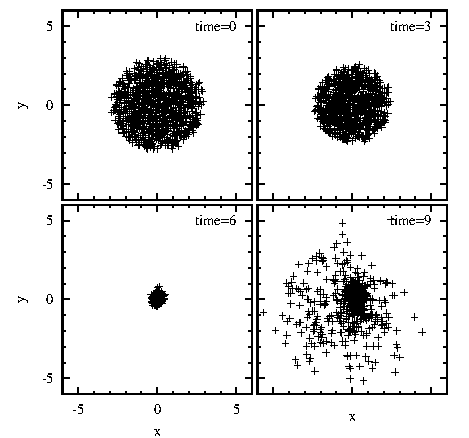
\includegraphics[width=0.75\linewidth]{fig/nbody.pdf}
\end{center}
\caption{}
\label{fig:nbody}
\end{figure}

\describeForEach{% C++用
粒子数を10000個にして計算を行いたい場合には以下のように実行すればよい(MPIを使用しない場合)。
\begin{screen}
\texttt{\$ ./nbody.out -N 10000}
\end{screen}
}{% Fortran用
粒子数を10000個にして計算を行いたい場合には、ファイル\texttt{f\_main.F90}の中のサブルーチン\texttt{f\_main()}のパラメータ変数\texttt{ntot}を10000に設定し、再度、コンパイルした上で実行すればよい。
}{%C言語用
粒子数を10000個にして計算を行いたい場合には、ファイル\texttt{c\_main.c}の中の関数\texttt{c\_main()}の変数\texttt{ntot}を10000に設定し、再度、コンパイルした上で実行すればよい。
}


%%%%%%%%%%%%%%%%
\subsubsubsection{x86版Phantom-GRAPEを使う場合}
\label{s3sec:phantom_grape_x86}
Phantom-GRAPEはSIMD命令を効率的に活用することで重力相互作用の計算を高速に実行するライブラリである(詳細はTanikawa et al.[2012, New Astronomy, 17, 82] とTanikawa et al.[2012, New Astronomy, 19, 74]を参照のこと)。

まず、使用環境を確認する。SIMD命令セットAVXをサポートするIntel CPUまたはAMD CPUを搭載したコンピュータを使用しているならば、x86版Phantom-GRAPEを使用可能である。

次にディレクトリ\texttt{\$(FDPS)/src/phantom\_grape\_x86/G5/newton/libpg5}に移動して、ファイル\texttt{Makefile}を編集し、コマンド\texttt{make}を実行してPhantom-GRAPEのライブラリ\texttt{libpg5.a}を作る。

最後に、ディレクトリ\dirNameNbodySample に戻り、ファイル\texttt{Makefile}内の\texttt{\\''\#use\_phantom\_grape\_x86 = yes''}の\texttt{''\#''}を消す。\texttt{make}を実行してコンパイルする(OpenMP, MPIの使用・不使用どちらにも対応)と、x86版Phantom-GRAPEを使用したコードができている。上と同様の方法で実行・結果の確認を行うとさきほどと同様の結果が得られる。

Intel Core i5-3210M CPU @ 2.50GHz の2コアで性能テスト(OpenMP使用、MPI不使用)をした結果、粒子数8192の場合に、Phantom-GRAPEを使うと、使わない場合に比べて、最大で5倍弱ほど高速なコードとなる。
\describeForCpp{%C++用
以下が最適化された実行例。
\begin{screen}
\texttt{\$ ./nbody.out -N 8192 -n 256}
\end{screen}
ここで、オプション「-n 数値」で相互作用リストを共有する粒子数の上限を指定している。
}

%%%%%%%%%%%%%%%%
\subsubsubsection{PIKGを使う場合}
\label{s3sec:pikg_x86}
PIKGはDSL(ドメイン固有言語)記述から様々なアーキテクチャ向けに最適化された粒子間相互作用カーネルを生成するカーネルジェネレータである.

ディレクトリ\dirNameNbodySample のファイル\texttt{Makefile}内の\texttt{\\''\#use\_pikg\_x86 = yes''}の\texttt{''\#''}を消す。
\describeForEach{% C++用
この状態で\texttt{make}を実行してコンパイルする(OpenMP, MPIの使用・不使用どちらにも対応)と、PIKGから生成されたカーネルを使用した実行ファイル\texttt{nbody.out}ができている。
}{% Fortran用
この状態で\texttt{make}を実行してコンパイルする(OpenMP, MPIの使用・不使用どちらにも対応)と、PIKGから生成されたカーネルを使用した実行ファイル\texttt{nbody.out}ができている。
}{% C言語用
この状態で\texttt{make}を実行してコンパイルする(OpenMP, MPIの使用・不使用どちらにも対応)と、PIKGから生成されたカーネルを使用した実行ファイル\texttt{nbody.out}ができている。
}
上と同様の方法で実行・結果の確認を行うとさきほどと同様の結果が得られる。

デフォルトでは,通常の \progLangName コードと同等の\texttt{reference}モードの相互作用カーネルが生成される.\texttt{Makefile}内の\texttt{\#COVERSION\_TYPE}とその直後にある
\describeForEach{\texttt{\#CFLAGS}}{\texttt{\#CXXFLAGS}}{\texttt{\#CXXFLAGS}}
の行のコメントアウトを外すと,別のアーキテクチャ(AVX2やAVX-512)向けにコードを生成できる.
AVX2モードを使う場合は,利用するCPUがAVX2及びFMAに対応していなくてはならない.さらにAVX-512モードを使う場合には利用するCPUがAVX-512FおよびAVX-512DQに対応していなくてはならない.

\ifCpp % C++用 (subsubsubsectionが1つ含まれている)
%%%%%%%%%%%%%%%%
\subsubsubsection{NVIDIAのGPUを使う場合}
\label{sec:use_nvidia_gpu}
サンプルにはCUDAによって書かれたNVIDIAのGPU用のカーネルも付属している。ディレクトリ\dirNameNbodySample の中のファイル\texttt{Makefile}内の\texttt{\\''\#use\_cuda\_gpu = yes''}の\texttt{''\#''}を消し、更に自分の環境に応じて、\texttt{CUDA\_HOME}の場所を設定する。\texttt{make}を実行してコンパイルする(OpenMP, MPIの使用・不使用どちらにも対応)と、GPUを使用したコードができている。上と同様の方法で実行・結果の確認を行うとさきほどと同様の結果が得られる。
\endifCpp

%%%%%%%%%%%%%%%%%%%%%%%%%%%%%%%
\subsubsection{SPHシミュレーションコード}
\label{subsubsec:usage_of_sample_codes:sph}
本サンプルコードには標準SPH法がFDPSを使って実装されている。簡単のため、smoothing lengthは一定値を取ると仮定している。コードでは、3次元の衝撃波管問題の初期条件を生成し、衝撃波管問題を実際に計算する。
%%%%%%%%%%%%%%%%
\subsubsubsection{概要}
以下の手順で本コードを使用できる。
\begin{itemize}
\item ディレクトリ\dirNameSPHSample に移動
\item カレントディレクトリにある\texttt{Makefile}を編集(後述)
\item コマンドライン上で\texttt{make}を実行
\item \texttt{sph.out}ファイルの実行(後述)
\item 結果の解析(後述)
\end{itemize}
%%%%%%%%%%%%%%%%
\subsubsubsection{ディレクトリ移動}
ディレクトリ\dirNameSPHSample に移動する。
%%%%%%%%%%%%%%%%
\subsubsubsection{Makefileの編集}
\describeForEach{% C++用
\texttt{Makefile}の編集の仕方は$N$体計算の場合と同一なので、 第\ref{s3sec:how_to_edit_Makefile_in_nbody}節を参照されたい。
}{% Fortran用
SPHサンプルコードにも、$N$体計算のサンプルコードの場合と同様、GCCとIntelコンパイラ用に2種類のMakefileが用意されている。編集の仕方は、$N$体計算の場合と同一なので、 第\ref{s3sec:how_to_edit_Makefile_in_nbody}節を参照されたい。
}{% C言語用
\texttt{Makefile}の編集の仕方は$N$体計算の場合と同一なので、 第\ref{s3sec:how_to_edit_Makefile_in_nbody}節を参照されたい。
}

%%%%%%%%%%%%%%%%
\subsubsubsection{\texttt{make}の実行}
\texttt{make}コマンドを実行する。
\describeForIF{% Fortran,C言語版
$N$体計算のときと同様、このとき、まずFDPSの\progLangName インターフェースプログラムが生成され、その後、インターフェースプログラムとサンプルコードが一緒にコンパイルされる。
}

%%%%%%%%%%%%%%%%
\subsubsubsection{実行}
実行方法は以下の通りである。
\begin{itemize}
\item MPIを使用しない場合、コマンドライン上で以下のコマンドを実行する
\begin{screen}
\begin{verbatim}
$ ./sph.out
\end{verbatim}
\end{screen}
  
\item MPIを使用する場合、コマンドライン上で以下のコマンドを実行する
\begin{screen}
\begin{verbatim}
$ MPIRUN -np NPROC ./sph.out
\end{verbatim}
\end{screen}
ここで、\texttt{MPIRUN}には\texttt{mpirun}や\texttt{mpiexec}などが、\texttt{NPROC}には使用するMPIプロセスの数が入る。
\end{itemize}

正しく終了すると以下のようなログを出力する。
\begin{screen}
\begin{verbatim}
******** FDPS has successfully finished. ********
\end{verbatim}
\end{screen}

%%%%%%%%%%%%%%%%
\subsubsubsection{結果の解析}
実行するとディレクトリ\texttt{result}にファイルが出力されている。
\describeForEach{% C++用
ファイル名は"00xx.txt"(xには数字が入る)となっている。ファイル名は時刻を表す。
}{% Fortran用
ファイル名は"snap0000x-proc0000y.dat" となっている。ここで、x,yは整数で、それぞれ、時刻とMPIプロセス番号を表す。MPI実行でない場合には、常にy=0である。
}{% C言語用
ファイル名は"snap0000x-proc0000y.dat" となっている。ここで、x,yは整数で、それぞれ、時刻とMPIプロセス番号を表す。MPI実行でない場合には、常にy=0である。
}
出力ファイルフォーマットは1列目から順に粒子のID、粒子の質量、位置のx, y, z座標、粒子のx, y, z軸方向の速度、密度、内部エネルギー、圧力である。

コマンドライン上で以下のコマンドを実行すれば、横軸に粒子のx座標、縦軸に粒子の密度をプロットできる(時刻は40)。
\ifCpp %C++用
\begin{screen}
\begin{verbatim}
$ gnuplot
$ plot "result/0040.txt" using 3:9
\end{verbatim}
\end{screen}
\endifCpp
\ifFtn %Fortran用
\begin{screen}
\begin{verbatim}
$ cd result
$ cat snap00040-proc* > snap00040.dat
$ gnuplot
> plot "snap00040.dat" using 3:9
\end{verbatim}
\end{screen}
\endifFtn
\ifC % C言語用
\begin{screen}
\begin{verbatim}
$ cd result
$ cat snap00040-proc* > snap00040.dat
$ gnuplot
> plot "snap00040.dat" using 3:9
\end{verbatim}
\end{screen}
\endifC
正しい答が得られれば、図\ref{fig:sph}のような図を描ける。

\begin{figure}[h]
\centering
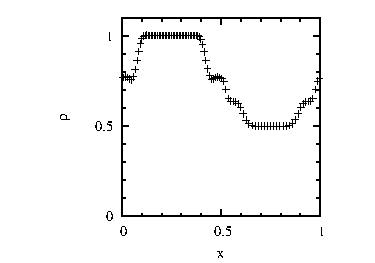
\includegraphics[width=0.5\linewidth]{fig/sph.pdf}
\caption{衝撃波管問題の時刻$t=40$における密度分布}
\label{fig:sph}
\end{figure}
